%\Large{Derivation of $\kappa$-rule and Net Production versions of energy
% allocation}

Let's call $F$ the functionnal response to the resource and $l$
the individual length. The energy intake $E_{in}$ of an individual
is a function of the functionnal response and the individual length:
\[
E_{in}=\epsilon\cdot F\cdot l^{2}
\]


where $\epsilon$ is a conversion coefficient. And the metabolism
is 
\[
\rho\cdot l^{3}
\]
 where $\rho$ is a parameter. 


\subsubsection*{$\kappa$-rule}

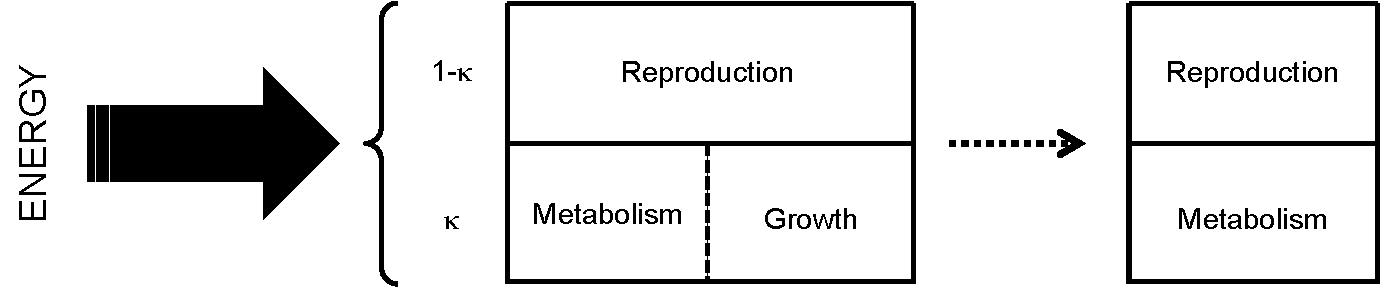
\includegraphics[width=0.95\textwidth]{4_ChapThe1/Fig/KRule}

In the $\kappa$-rule, the energy intake (thick black arrow) is first
divided into $1-\kappa$ allocated to reproduction and $\kappa$ allocated
to metabolism, and if all the metabolism cost is paid, the rest of
this $\kappa$ fraction goes to growth. Once the individual has reached
it's maximum size (dashed arrow), the energy intake is allocated to
the metabolism and the rest to reproduction. We not that even after
reaching its maximum size, an individual continues to reproduce until
it cannot fulfill its metabolism anymore and dies.

Given the rules of energy allocation, we can write the individual
growth rate and reproduction rate as functions of the functional response
and the individual length.

Birth rate represents the production of newborns (mass or weight $w$)
from the energy absorbed, and can be written:
\begin{eqnarray*}
b_{\kappa}(l) & = & (1-\kappa)\cdot\epsilon\cdot Fl^{2}\\
 & = & r_{m}\cdot Fl^{2}
\end{eqnarray*}


where $r_{m}=(1-\kappa)\cdot\epsilon$ is a reproduction rate. We
note that the birth rate increases with body length following a parabola. 

As opposed to reproduction which is an increase in weight, growth
is the increase in body length $l$. We then define the parameter
$c$ as a length to weight coefficient such as $w=c\cdot l^{3}$,
which leads to 
\[
\frac{dw}{dl}=3c\cdot l^{2}\Leftrightarrow\frac{dl}{dw}=\frac{1}{3cl^{2}}
\]


Expressed in words, growth rate is the fraction $\kappa$ of the energy
intake minus the cost of metabolism. That is to say:

\[
g_{\kappa}(l)=\frac{dl}{dt}=\frac{dw}{dt}\cdot\frac{dl}{dw}=\frac{1}{3cl^{2}}\cdot\frac{dw}{dt}
\]


where $\frac{dw}{dt}$, the change in weight over time is 
\[
\frac{dw}{dt}=\kappa\cdot\epsilon\cdot Fl^{2}-\rho l^{3}
\]
The growth rate in body length is then 
\begin{eqnarray*}
g_{\kappa} & = & \frac{1}{3cl^{2}}\cdot\left(\kappa\cdot\epsilon\cdot Fl^{2}-\rho l^{3}\right)\\
 & = & \frac{1}{3c}\cdot\left(\kappa\cdot\epsilon\cdot F-\rho l\right)\\
 & = & \frac{\rho}{3c}\cdot\left(\frac{\kappa\epsilon}{\rho}F-l\right)
\end{eqnarray*}
Let's define ${\displaystyle \gamma=\frac{\rho}{3c}}$ and ${\displaystyle L_{M}=\frac{\kappa\epsilon}{\rho}}$,
respectively the von Bertalanffy growth parameter and the absolute
maximum length, that is to say the length at infinite resources and
without competition, we can then write the growth rate in the case
of the $\kappa$-rule as follows:

\[
g_{\kappa}(l)=\gamma\cdot\left(L_{M}\cdot F-l\right)
\]


which integrates as the von Bertalanffy growth function for an isolated
individual. We can see that with the biological interpretations of
$\gamma$ and $L_{M}$, we don't need to have access to the value
of $\kappa$ to parametrize the model.


\subsubsection{The net production model}

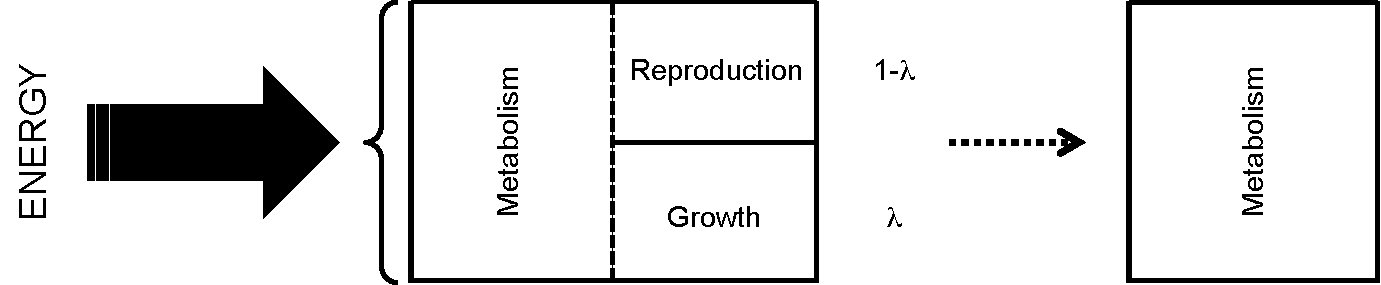
\includegraphics[width=0.95\textwidth]{4_ChapThe1/Fig/NPRule}

In the net production model, the energy intake is first allocated
to metabolism. If some energy is left after fulfilling metabolism,
the energy is divided between growth (fraction $\lambda$) and reproduction
(fraction $1-\lambda$). Once the individual stops growing, meaning
it can only fulfill its metabolism, it stops reproducing at the same
time.

Given the rules of energy allocation, we can write the individual
growth rate and reproduction rate as functions of the functional response
and the individual length.

As before, the growth rate in body length can be written as follows:
\[
g_{\text{NP}}=\frac{1}{3cl^{2}}\cdot\frac{dw}{dt}
\]


where $\frac{dw}{dt}$, the change in wheight over time is a fraction
$\lambda$ of what is left after paying for the metabolism: 
\[
\frac{dw}{dt}=\lambda\cdot\left(\epsilon\cdot Fl^{2}-\rho l^{3}\right)
\]


We can hence write the growth rate as follows:
\begin{eqnarray*}
g_{\text{NP}} & = & \frac{1}{3cl^{2}}\cdot\lambda\cdot\left(\epsilon\cdot Fl^{2}-\rho l^{3}\right)\\
 & = & \lambda\cdot\frac{1}{3c}\cdot\left(\epsilon\cdot F-\rho l\right)\\
 & = & \lambda\cdot\frac{\rho}{3c}\cdot\left(\frac{\epsilon}{\rho}F-l\right)
\end{eqnarray*}


Using ${\displaystyle \xi=\lambda\frac{\rho}{3c}}$ and ${\displaystyle L_{NP}=\frac{\epsilon}{\rho}}$
as the von Bertalanffy growth parameter and the absolute maximum length,
we can write the growth rate as:
\[
g_{\text{NP}}(l)=\xi\cdot\left(L_{NP}\cdot F-l\right)
\]


We see that $g_{\kappa}$ and $g_{\text{NP}}$ have the exact same
form. Although the definition of the parameters differ, their biological
interpretation remain the same, with respectively $\gamma$ and $\xi$
the von Bertalanffy growth parameters and $L_{M}$ and $L_{NP}$ the
absolute maximum length. 

As previously, the birth rate is the increase in mass of newborns:
\[
b_{\text{NP}}(l)=\frac{dw}{dt}\cdot\frac{1}{\omega}
\]
where $\omega$ is the weight of on newborn. With the net production
model, the birth rate is the fraction $1-\lambda$ of the energy left
after fulfilling metabolism:
\begin{eqnarray*}
b_{\text{NP}}(l) & = & \frac{1}{\omega}\cdot(1-\lambda)\cdot\left(\epsilon\cdot Fl^{2}-\rho l^{3}\right)\\
 & = & \frac{1}{\omega}\cdot(1-\lambda)\cdot\rho l^{2}\cdot\left(\frac{\epsilon}{\rho}\cdot F-l\right)
\end{eqnarray*}


Multiplying by $\frac{\lambda}{\lambda}$ we can identify the growth
function $g_{\text{NP}}$:

\begin{eqnarray*}
b_{\text{NP}}(l) & = & \frac{3c}{\omega}\cdot(1-\lambda)\cdot\underbrace{\frac{\lambda}{\lambda}\cdot\frac{\rho}{3c}\cdot\left(\frac{\epsilon}{\rho}\cdot F-l\right)}\cdot l^{2}\\
 & = & \frac{3c}{\omega}\cdot\frac{(1-\lambda)}{\lambda}\cdot\qquad\quad g_{\text{NP}}(l)\;\qquad\cdot l^{2}
\end{eqnarray*}


Furthermore, with $w=3c\cdot l^{3}$, we can write $\omega=c\cdot L_{b}^{3}$
where $L_{b}$ is the body length at birth. We then have:
\begin{eqnarray*}
b_{\text{NP}}(l) & = & \frac{(1-\lambda)}{\lambda}\cdot\frac{3}{L_{b}^{3}}\cdot g_{\text{NP}}(l)\cdot l^{2}
\end{eqnarray*}


We define the parameter ${\displaystyle \beta=\frac{(1-\lambda)}{\lambda}\cdot\frac{3}{L_{b}^{3}}}$,
and the birth rate writes as
\[
b_{\text{NP}}(l)=\beta\cdot g_{\text{NP}}(l)\cdot l^{2}
\]


We can see that this time that the birth rate is a third degree polynom
which first increases with $l$, and then decreases to $0$ when the
individuals stops growing at $l=L_{M}\cdot F$.

Going a little further, $g_{\text{NP}}$ is maximum for $l=0$ and
$F=1$ and is equal to $g_{\text{NP}}=\xi\cdot L_{NP}$. Hence, if
we write ${\displaystyle G(l)=\frac{g_{\text{NP}}(l)}{\xi\cdot L_{NP}}}$
and ${\displaystyle \beta^{'}=\xi\cdot L_{NP}\cdot\beta}$, we obtain
\[
b_{\text{NP}}(l)=\beta^{'}\cdot G(l)\cdot l^{2}
\]
 where $G$ scales from $0$ to $1$.


\subsubsection{From one rule to the other}

In our model, we used the $\kappa$-rule with parameters $\gamma$
and $L_{M}$ estimated using data from experiments on the collembolan
\textit{Folsomia candida. }The parameter $L_{b}$ is also estimated
using the same experiments. To convert the model to a net production
energy allocation rule, we can keep the same equation for the growth
function, and simply estimate $\lambda$ which will give a value $\beta$,
knowing the length at birth $L_{b}$. But $\lambda$ is very difficult
to estimate properly. 

To decide which of the two rules are best suited to fit experimental
or empirical data, one can look at the reproduction rate or the fecundity
as a function of body length. A continuously growing fecundity with
body length is an indication that the $\kappa$-rule is more fit for
the data, wheras a bell-shaped form would tend to a net production
model for the energy allocation. 

In the case of the collembola \textit{Folsomia candida}, measures
on isolated individuals shows that the reproduction rate is positively
correlated with body length, which suggests the net production model
is not adapted and the $\kappa$-rule should be used as a dynamic
energy budget rule for this system.